\section*{Lectura 11: El Grupo Fundamental.}

\begin{definition}
    Sea $X$ un espacio topologico y  $f:[0,1] \xrightarrow{} X$ y $g:[0,1]
    \xrightarrow{} X$ caminos en $X$ con  $f(1)=g(0)$. Definimos el
    \textbf{(roducto de caminos} de ser la operacion binaria $\ast$ que lleva
    $(f,g) \xrightarrow{} f \ast g$ tal que
    \begin{equation*}
        f \ast g(t)=\begin{cases}
                f(2t), & \text{ s\'i } 0 \leq t \leq \frac{1}{2}    \\
                g(2t-1), & \text{ \s'i } \frac{1}{2} \leq t \leq 1  \\
            \end{cases}
    \end{equation*}
\end{definition}

\begin{lemma}\label{11.31}
    El producto de caminos es una mapa continua.
\end{lemma}
\begin{proof}
    Esto sigue del teorema del empaste.
\end{proof}
\begin{corollary}
    El producto de caminos es un camino.
\end{corollary}

\begin{definition}
    Sea $X$ un espacio topologico, y  $A$ subespacio de  $X$. Sean  $f_0:X
    \xrightarrow{} Y$ y $f_1:X \xrightarrow{} Y$ mapas continuas con
    $f_0|_A=f_1|_A$. Decimos que $f_0$ es \textbf{relativamente homotopico} a
    $f_1$, relativo a $A$ s\'i existe una mapa continua $F:X \times [0,1]
    \xrightarrow{} Y$ tal que $F:f_0 \simeq f_1$ y $F(a,t)=f_0(a)=f_1(a)$ para
    todo $a \in A$. Escribimos  $f_0 \simeq f_1 \rel{A}$ y llamamos a $F:f_0
    \simeq f_1 \rel{A}$ la \textbf{homotopia relativa} entre $f_0$ y $f_1$.
\end{definition}

\begin{example}\label{}
    Sea $X$ un espacio topologico y  $A=\emptyset$. Entonces la relacion  $f_0
    \simeq f_1 \rel{A}$ es nada mas que la homotopia usual $f_0 \simeq f_1$.
    Llamamos a este homotopia relativa la \textbf{homotopia libre}.
\end{example}

\begin{lemma}\label{11.32}
    La relacion $\simeq_A$ de homotopia relativa es una relacion de
    equivalencia.
\end{lemma}

\begin{figure}[h]
    \centering
    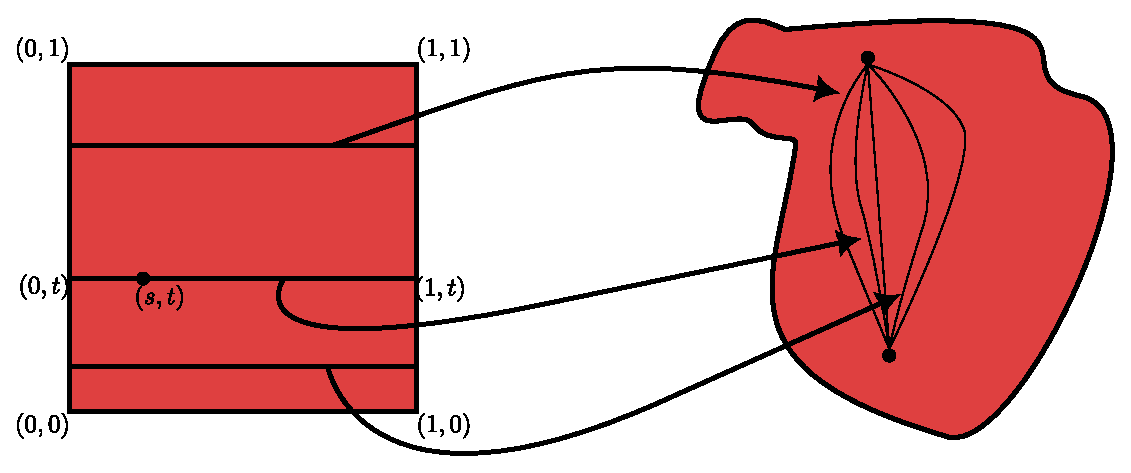
\includegraphics[scale=0.5]{Figures/path_prod.eps}
    \caption{Una homotopia relativa entre caminos.}
    \label{fig_21}
\end{figure}

\begin{definition}
    Sea $\partial{I}$ el borde de $I=[0,1]$. Llamaos las clases de equivalencias
    de la homotopia relativa $\simeq_{\partial{I}}$ \textbf{clases de caminos}.
    S\'i $f$ es un camino, denotamos el clase de caminos de  $f$ por  $[f]$.
\end{definition}

\begin{theorem}\label{11.32}
    Suponga que $f_0,f_1$ y $g_0,g_1$ son caminos en un espacio topologico $X$
    tales que  $f_0 \simeq f_1 \rel{\partial{I}}$ y $g_0 \simeq g_1
    \rel{\partial{I}}$. S\'i $f_0(1)=g_0(0)$ y $f_1(1)=g_1(0)$, entonces
    $f_0 \ast g_0 \simeq f_1 \ast g_1 \rel{\partial{I}}$.
\end{theorem}
\begin{proof}
    Sean $F:f_0 \simeq f_1 \rel{\partial{I}}$ y $G:g_0 \simeq g_1
    \rel{\partial{I}}$ homotopias relativas entres  $f_0$ y $f_1$, y $g_0$ y
    $g_1$. Defina la mapa $H:[0,1] \times [0,1] \xrightarrow{} Y$ dado por
    \begin{equation*}
     H(s,t)=\begin{cases}
                 F(2s,t), & \text{ s\'i } 0 \leq s \leq \frac{1}{2} \\
                 G(2s-1,t), & \text{ s\'i } \frac{1}{2} \leq s \leq 1   \\
            \end{cases}
    \end{equation*}
    Por el teorema del empaste, vemos que $H$ es continua, ademas vemos que
    $H(0,t)=F(0,t)=f_0 \ast g_0(t)$, y $H(1,t)=G(1,t)=f_1 \ast g_1(t)$. As\'i
    que $H:f_0 \ast g_0 \simeq f_1 \ast g_1 \rel{\partial{I}}$ es una homotopia
    relativa.
\end{proof}
\begin{corollary}
    $[f_0 \ast g_0]=[f_1 \ast g_1]$.
\end{corollary}

\begin{definition}
    S\'i $f:[0,1] \xrightarrow{} X$ es un camino con $x_0=f(0)$ y $x_1=f(1)$,
    entonces llamaos a $x_0$ el \textbf{origen} y $x_1$ el \textbf{final} de
    $f$, y lo denotamos por  $x_0=\alpha(f)$ y $x_1=\omega(f)$. Denotamos el
    origen y final del clase de caminos de ser $\alpha[f]=\alpha([f])$ y
    $\omega[f]=\omaga([f])$, respectivamente.
\end{definition}

\begin{definition}
    S\'i $f:[0,1] \xrightarrow{} X$ es un camino y $p$ es un punto en  $X$,
    entonces llamamos la mapa constante  $i_p:t \xrightarrow{} p$, para todo $t
    \in [0,1]$ el \textbf{camino constante}. Similarmente, llamamos al la mapa
    $\inv{f}(t)=f(1-t)$ el \textbf{camino inverso} de $f$.
\end{definition}

\begin{definition}
    Llamamos a un conjunto $G$, junto a una operacion binaria $\ast$ (no
    siempre definida) un \textbf{grupoide} s\'i
    \begin{enumerate}
        \item[(1)] $a \ast (b \ast c)=(a \ast b) \ast c$ s\'i $a \ast (b \ast
            c)$, o $(a \ast b) \ast c$ estan definidos, para todo $a,b,c \in G$.

        \item[(2)] Existen elementos $e_1,e_2 \in G$ tal que $a \ast e_1=a$ y
            $e_2 \ast a=a$; para todo $a \in G$.

            \item[(3)] Para toda $a \in G$, existe un elemento  $\inv{a} \in G$
                tal que $a \ast \inv{a}=e_1$ y $\inv{a} \ast a=e_2$.
    \end{enumerate}
\end{definition}

\begin{theorem}\label{11.34}
    S\'i $X$ es un espacio topologico, entonces el conjunto de todas las clases
    de caminos de  $X$ forman un grupoide bajo el producto de caminos. Es decir:
    \begin{enumerate}
        \item[(1)] El producto de caminos es associativa cuando esta definido
            apropiadamente.

        \item[(2)] S\'i $p=\alpha[f]$ y $q=\omega[f]$, entonces existen caminos
            constantes $i_p$ y $i_q$ tales que
            \begin{align*}
                [i_p][f]=f  &&  \text{y}   &&   [f][i_q]=[f]       \\
            \end{align*}

        \item[(3)] Para todo clase de camio $[f]$, existe el clase de camino
        $[\inv{f}]$ es tal que:
            \begin{align*}
                [f][\inv{f}]=[i_p]  &&  \text{y}    &&  [\inv{f}][f]=[i_q]  \\
            \end{align*}
            donde $p=\alpha[f]$ y $q=\omega[f]$.
    \end{enumerate}
\end{theorem}
\begin{proof}
    Dado $a,b \in \R$, defina la mapa $\theta_{[a,b]}:[a,b] \xrightarrow{}
    [0,1]$ dado por la regla
    \begin{equation*}
        \theta_{[a,b]}(s)=\frac{s-a}{b-a} \text{ para todo } s \in [a,b]
    \end{equation*}
    $\theta_{[a,b]}$ es una aplicaci\'on af\'in para todo $a,b \in \R$. Nota que
     $\theta_{[a,b]}(a)=0$ y $\theta_{[a,b]}(b)=1$. Mas a\'un, para cualquier
     camino $f$,  $f \circ \theta_{[a,b]}$ es continua.

     Sea $f:I \xrightarrow{} X$, $g:I \xrightarrow{} X$, y $h:I \xrightarrow{}
     X$ caminos donde $f(1)=g(0)$, $g(1)=h(0)$ y $(f \ast g) \ast h$, o $f \ast
     (g \ast h)$ estan definidos y considere la figura \ref{fig_22}.
     \begin{figure}[h]
         \centering
         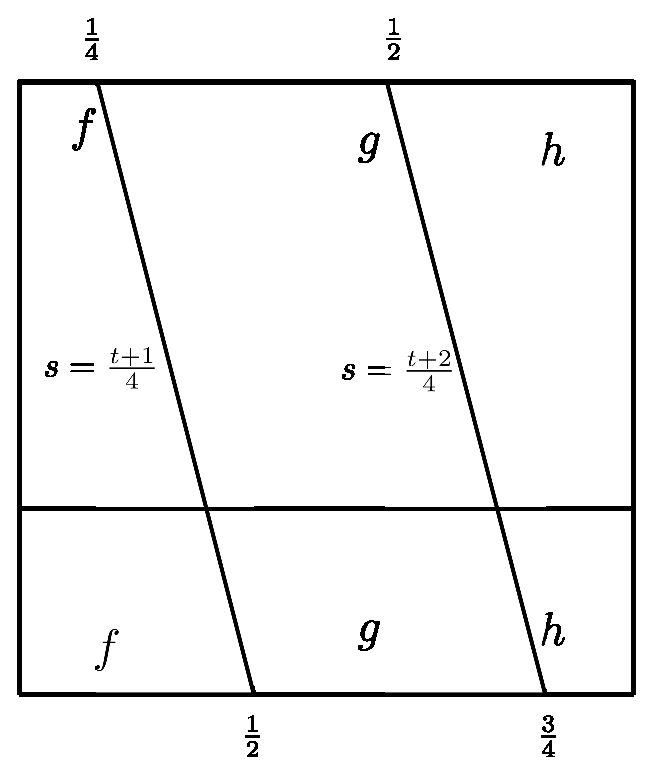
\includegraphics[scale=0.5]{Figures/path_associativity.eps}
         \caption{}
         \label{fig_22}
     \end{figure}
     Defina $H:I \times I \xrightarrow{} X$ dado por
     \begin{equation*}
          H(s,t)=\begin{cases}
                    f(\frac{4s}{1+t}), & \text{ s\'i } s \in [0,\frac{t+1}{4}] \\
                    g(4s-1-t), & \text{ s\'i } s \in [\frac{t+1}{4},\frac{t+2}{4}]   \\
                    h(1-\frac{4(1-s)}{2-t}), & \text{ s\'i } s \in [\frac{t+2}{4},1] \\
                 \end{cases}
     \end{equation*}
     $H$ es continua por el teorema del empaste. Mas a\'un $H(s,0)=(f \ast g)
     \ast h(s)$ y $H(s,1)=f \ast (g \ast h)(s)$. Por ultimo $H(0,t)=f(0)=p$ y
     $H(1,t)=h(1)=q$. Por lo tanto $(f \ast g) \ast h \simeq f \ast (g \ast h)
     \rel{partial{I}}$.

     Ahora, sea $[f]$ una clase de camino de $X$ con  $p=\alpha[f]$ y
     $q=\omega[f]$. Sean $i_p:t \xrightarrow{} p$ y $i_q:t \xrightarrow{} q$ los
     caminos constantes correspondiente a $p$ y $q$. Considere el sigueinte
     figura \ref{fig_23}

     \begin{figure}[h]
         \centering
         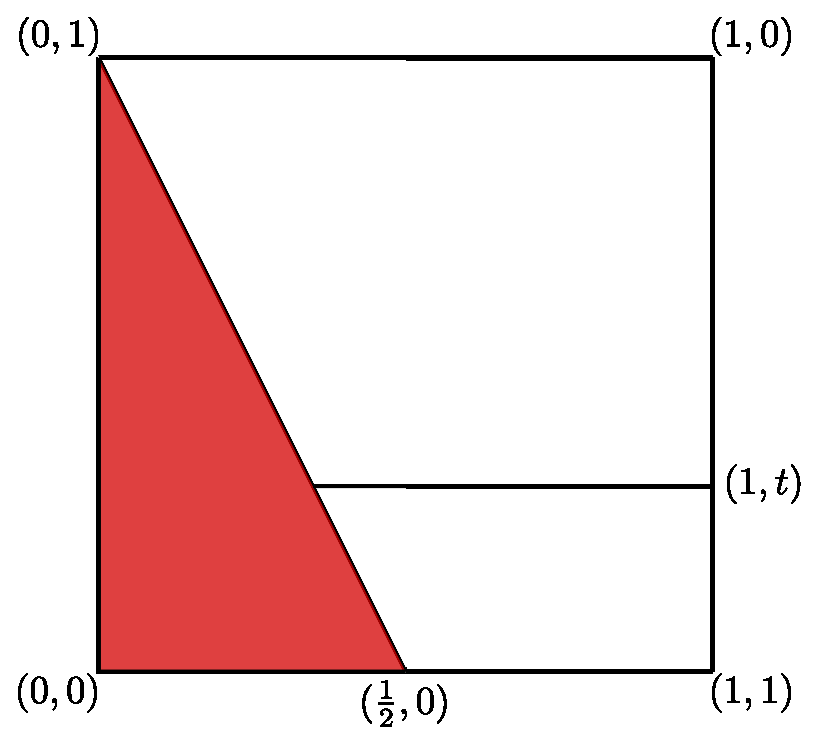
\includegraphics[scale=0.5]{Figures/path_identity.eps}
         \caption{}
         \label{fig_23}
     \end{figure}

     Defina la mapa $H:I \times I \xrightarrow{} X$ dado por
     \begin{equation*}
          H(s,t)=\begin{cases}
                    p, & \text{ s\'i } s \in [0,\frac{t}{2}]    \\
                    f(\theta_{[\frac{t}{2},1]}(s)), & \text{ s\'i } s \in
                    [\frac{t}{2},1]
                 \end{cases}
     \end{equation*}
     Note que $H(\frac{t}{2},t)=f(0)=p$, as\'i por el teorema del empaste, $H$
     es continua. Mas a\'un nota que $H(s,0)=f(s)$ y $H(s,1)=i_p \ast f$. Vemos
     tambien que $H(0,t)=p$ y $H(1,t)=f(1)=q$. Por lo tanto $i_p \ast f \simeq f
     \rel{\partial{I}}$. De igual manera, podemos ver que $f \ast i_q \simeq f
     \rel{\partial{I}}$.

     Por ultimo, sea $f$ un camino en $X$ con $p=\alpha(f)$ y $q=\omega(f)$.
     Considere el camino inverso $\inv{f}$, y construye la figura \ref{fig_24}.
     \begin{figure}[h]
         \centering
         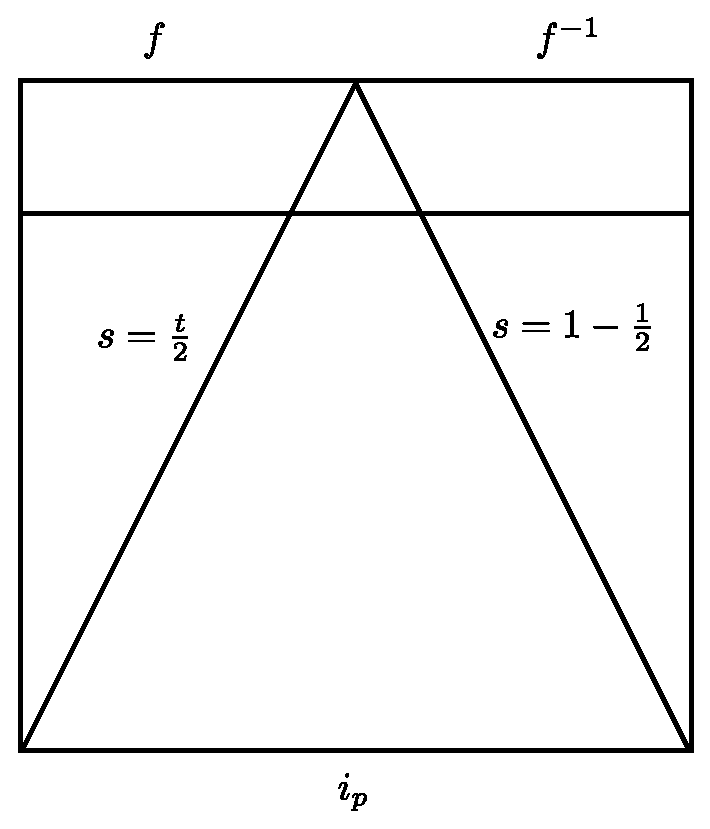
\includegraphics[scale=0.5]{Figures/path_inverse.eps}
         \caption{}
         \label{fig_24}
     \end{figure}
    Defina $H:I \times I \xrightarrow{} X$ por
    \begin{equation*}
          H(s,t)=\begin{cases}
                      f(2s), & \text{ s\'i } s \in [0, \frac{t}{2}]  \\
                      f(t), & \text{ s\'i } s \in [\frac{t}{2}, \frac{1-t}{2}] \\
                      \inv{f}(2(1-s)), &  \text{ s\'i } s \in [\frac{1-t}{2},1]  \\
                 \end{cases}
    \end{equation*}
    Nota que $H$ es continua por empaste. Mas a\'un, $H(s,0)=f(0)=p=i_p(s)$ y
    $H(s,1)=f \ast \inv{f}(s)$. Mas a\'un $H(0,t)=f(0)=p$ y
    $H(1,t)=\inv{f}(0)=q$. As\'i que $f \ast \inv{f} \simeq i_p
    \rel{\partial{I}}$. Similarmente, se halla que $\inv{f} \ast f \simeq i_q
    \rel{\partial{I}}$.
\end{proof}
